\TODO{the annotation of tuples is encoded as an attribute in implementation.}
\TODO{fix the fig}

%\point{vdb and vschema and config (bottom of fig).}
%\textbf{VDBMS architecture:}
\figref{arch} shows the architecture of VDBMS and its modules.
For now, we assume a VDB and its v-schema are generated by an 
expert and are stored in a DBMS, we provide guidelines and case studies of
systematically generating VDBs in 
\secref{db}. A VDB can be \emph{configured} to its pure relational 
database variants, if desired by a user, by providing the configuration
of the desired variant, \figref{vdb-conf}.
For example, a SPL developer configures a VDB to produce 
software and its database for a client.
%To configure a VDB, VDBMS requires a list of valid configurations.
%Remember that the feature model is a feature expression that 
%encodes all valid configurations. Hence, solving the feature model
%by a SAT solver results in the list of valid configurations.

%\point{flow of vq in vdbms.}
Given a VDB and its v-schema, a user inputs a v-query \vQ\ to VDBMS.
%
First, \vQ\ is checked by the \emph{type system} to determine if it is invalid, explained in 
%First, \vQ\ is type-checked by the VRA type system introduced in 
\secref{type-sys}. 
If so, the user gets errors explaining what part of the 
query violated the v-schema.
%, shown in \exref{q-violate-sch}.
%\moredet{maybe give an ex of an error user will see! ref to ex of error given
%in \secref{type-sys}}
Otherwise, 
\vQ\ is explicitly annotated with the schema,
defined in \secref{constrain},
to ensure variation-preserving property w.r.t. v-schema throughout the execution flow of v-query 
in the system and then
%
it is passed to the \emph{variation minimization} module, introduced in 
\secref{var-min}, to minimize the variation of \vQ\ and apply
relational algebra optimization rules. 
%
The optimized query is then sent to the \emph{generator} module where
SQL queries are generated from v-queries, \secref{apps} provides three
approaches for this.
\TODO{fix this!!}
%\exref{q-flow} in \appref{sql-gen} demonstrates the flow of a v-query through
%VDBMS.

\begin{comment}
To generate runnable queries w.r.t. the underlying DBMS,
the minimized query \ensuremath {\VVal \vQ} is passed to 
the \emph{translate to RA} module that could use either 
configuring or grouping of v-queries, explained in \secref{vra-sem},
to generate RA queries. The generated 
queries are then sent to the \emph{SQL generator} module which generates
SQL queries in various ways from the relational algebra queries, explained
in \secref{sql-gen}.
%\moredet{in app have an ex of all this happening!}
\end{comment}

%\point{vtab builder.}
Having generated SQL queries, they are now run over the underlying 
VDB (stored in a DBMS desired by the user). The result could be either 
a v-table or a list of v-tables, depending on the approach chosen in 
the translator to RA and SQL generator modules. The v-table(s) is passed
to the \emph{v-table builder}
%\dropit{could drop \secref{vtab-build} and explain it here!}
%explained in \secref{vtab-build}, 
to create one v-table that filters out 
duplicate and invalid tuples, shrinks presence conditions, and 
eventually, returns the final v-table to the user.

\begin{figure}
\centering
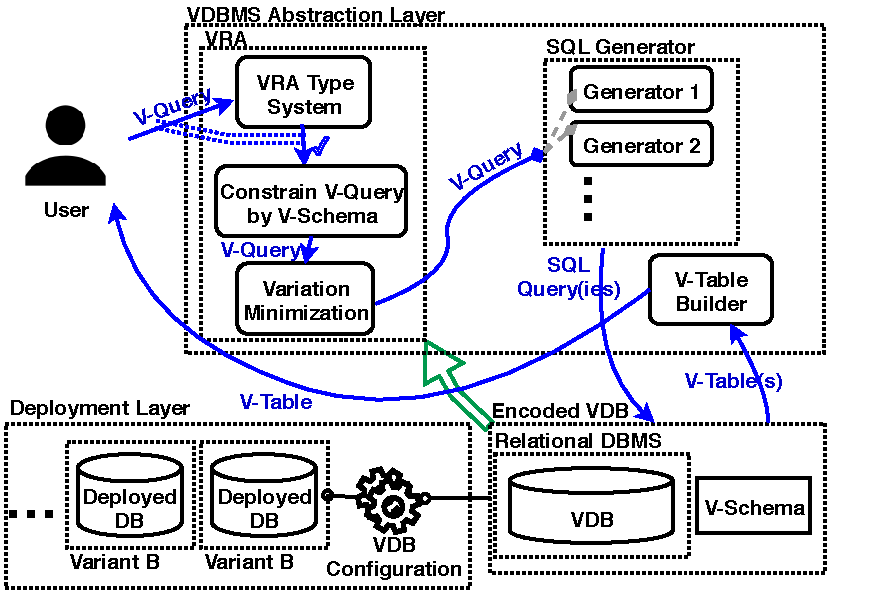
\includegraphics[scale = 0.7] {figs/arch7.pdf}
\caption{VDBMS architecture and execution flow of a v-query. 
The dotted double-line from v-query to pushing v-schema module
indicates the dependency of passing the v-query to this module
only if it is valid. 
The dashed gray arrows with diamond heads demonstrate
an option for the flow of input. 
%We examine taking different routes
%to evaluate a v-query, resulting in various approaches in \secref{apps}.
The blue filled arrows track the data flow, the green hollow arrows 
indicate an input to a module.}
\label{fig:arch}
\end{figure}


